\begin{landscape}
    \null\vfill
    \begin{figure}[htbp]
        \centering
        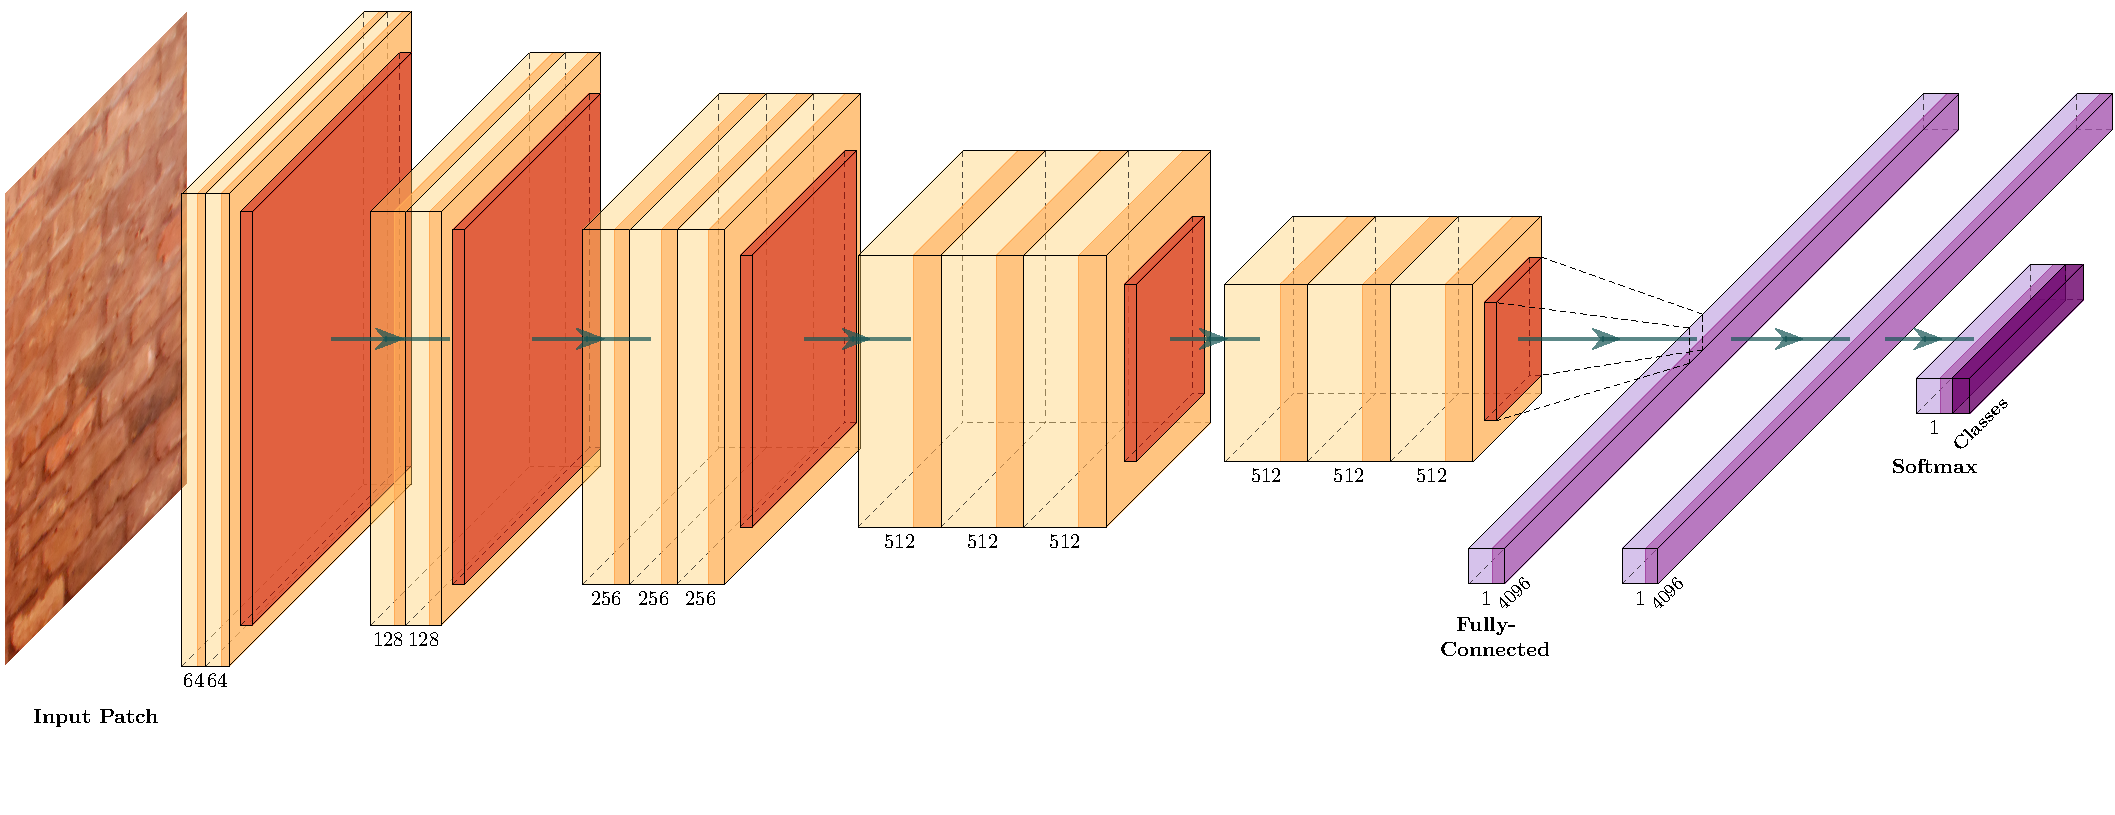
\includegraphics[width=0.95\linewidth]{chi-model}
        \caption[Texture-based acoustic material tagging model]{Unlike the image-to-image model used for the camera-based material tagging system, the texture-based approach outputs semantic classes based on an input image patch. The system extract image patches from textures associated with objects in the virtual environment. Output classes are then used to create acoustic materials via semantic mappings.}\label{fig:chi-model}
    \end{figure}
    \null\vfill
\end{landscape}